% !TEX root = cikm2018-visual-ltr.tex

\section{The \protect\datasetname{} Data\-set}
\label{sec:dataset}
%In this section, we describe the \datasetname~data\-set. 
\if0
Section~\ref{sec:trecclue} contains information about the underlying ClueWeb12 collection and TREC Web Track topics. Section~\ref{sec:screenshotsec} explains how the snapshots for ClueWeb12 were acquired using the Wayback Machine\footnote{\url{http://archive.org/web/}} and ClueWeb12 Online rendering service.\footnote{\url{http://boston.lti.cs.cmu.edu/Services/}} Section~\ref{sec:contentfeature} discusses the details on how content features, such as BM25 and TF-IDF, are calculated using Apache Spark.\footnote{\url{https://spark.apache.org/}} Finally, Section~\ref{sec:finalcollection} gives an overview of the structure in which the \datasetname~dataset is presented.
\fi

\subsection{ClueWeb12 \& TREC Web Track}\label{sec:trecclue}
For \datasetname{} we choose to use a combination of the ClueWeb12 document collection and the topics from the TREC Web Tracks 2013 \& 2014~\cite{collins2013trec,collins2015trec},
because this is currently the most recent combination of a large-scale web page collection together with judged queries (with graded relevance). 

ClueWeb12 is a highly diverse collection of web pages scraped in the first half of 2012.
The total collection contains over 700 million documents that are crawled using the typical crawling settings of the Heritrix archival crawler project.\footnote{\url{https://webarchive.jira.com/wiki/spaces/Heritrix/overview}}

We only use ClueWeb12 documents that have been judged for any of the 100 queries in the TREC Web Tracks 2013 \& 2014. In total, there are 28,906 judged pages.
%
Table~\ref{tab:countsources} shows the breakdown of the total number of pages and different relevance labels in the combined set of topics from 2013 and 2014.


\begin{table}[h]
  \captionof{table}{The total number of documents per source and the corresponding breakdown of  TREC Web Track relevance grades.} 
%  \captionof{table}{A breakdown of the relevance judgments for the TREC Web Tracks and the number of snapshots taken from the Wayback Machine and ClueWeb12 rendering service.} 
  \label{tab:countsources}
  \begin{tabular}{ l  @{}r  r  r  r }
  \toprule
    Count/Label & TREC Web & Wayback & ClueWeb12 & \mbox{}\hspace*{-.15cm}No image\\
    \midrule
    Total & 28,906 & 23,249 & 5,392 & 265 \\
    Nav grade (4) & 40 & 36 & 4 & 0\\
    Key grade (3) & 409 & 347 & 62 & 0\\
    Hrel grade (2) & 2,534 & 2,222 & 295 & 17 \\
    Rel grade (1) & 6,832 & 5,679 & 1,123 & 30\\
    Non grade (0) & 18,301 & 14,395 & 3,701 & 205 \\
    Junk grade (-2) & 790 & 570 & 207 & 13\\
    \bottomrule
  \end{tabular} 
\end{table}


\subsection{Snapshots} \label{sec:screenshotsec}
%
%\begin{table*}[t]
%\begin{center}
%\begin{tabular}{llllllll}
%\multicolumn{8}{c}{Clueweb12 11 features}                                    \\ 
%                      & P@1   & P@5   & P@10  & NDCG@1 & NDCG@5 & NDCG@10 & MAP   \\ \hline
%BM25                  & 0.300 & 0.319 & 0.316 & 0.153  & 0.197  & 0.188   & 0.350 \\ \hline
%RankBoost             & 0.420 & 0.432 & 0.441 & 0.244  & 0.270  & 0.285   & 0.423 \\
%AdaRank               & 0.260 & 0.362 & 0.377 & 0.132  & 0.203  & 0.228   & 0.383 \\
%LambdaMart            & 0.440 & 0.442 & 0.467 & 0.243  & 0.268  & 0.294   & 0.434 \\ \hline
%ViP baseline          & 0.338 & 0.359 & 0.370 & 0.189  & 0.215  & 0.233   & 0.415 \\ \hline
%%ViP masks             & 0.346 & 0.391 & 0.399 & 0.186  & 0.232  & 0.251   & 0.419 \\
%ViP highlights        & 0.418 & 0.409 & 0.416 & 0.239  & 0.253  & 0.269   & 0.422 \\
%ViP snapshots         & 0.392 & 0.389 & 0.398 & 0.217  & 0.238  & 0.254   & 0.421 \\ \hline
%VGG snapshots      & 0.514 & 0.488 & 0.484 & 0.292  & 0.307  & 0.324   & 0.442 \\ 
%VGG highlights     & 0.560 & 0.547 & 0.520 & 0.323  & 0.337  & 0.346   & 0.456 \\ \hline
%VGG saliency       & 0.554 & 0.478 & 0.453 & 0.310  & 0.296  & 0.302   & 0.422 \\
%\end{tabular}
%\centering
%\captionof{table}{Results after 5 iterations on all 5 folds of \datasetname. ViP is the model by \citet{fan2017learning}, the baseline uses only content features and VGG-16 is the pre-trained feature extractor.}
%\label{tab:results}
%\end{center}
%\end{table*}

%\begin{table*}[h]
%\caption{A benchmark comparison between the MQ2007 query set using all 46 LETOR features and the 11 LETOR features that are used in \datasetname.}
%\label{tab:11vs46}
%\centering
%\begin{tabular}{lccccccc}
%\toprule
%%& \multicolumn{7}{c}{MQ2007 46 features vs 11 features}                                     \\
%           & P@1    & P@5    & P@10   & NDCG@1 & NDCG@5 & NDCG@10 & MAP    \\ 
%\midrule
%RankBoost - 46  & 0.453 & 0.404 & 0.371 & 0.391 & 0.403 & 0.430  & 0.457 \\
%RankBoost - 11 & 0.448 & 0.400 & 0.372 & 0.381  & 0.401  & 0.431   & 0.453 \\
%\midrule
%AdaRank - 46  & 0.420 & 0.402 & 0.360 & 0.367 & 0.403 & 0.424  & 0.449 \\
%AdaRank - 11  & 0.385 & 0.391 & 0.287 & 0.364  & 0.396  & 0.394   & 0.386 \\ 
%\midrule
%LambdaMart - 46 & 0.452 & 0.418 & 0.384 & 0.405 & 0.411 & 0.444  & 0.463 \\
%LambdaMart - 11 & 0.448 & 0.412 & 0.380 & 0.397  & 0.411  & 0.443   & 0.455 \\
%\bottomrule
%\end{tabular}
%\end{table*}

%\subsubsection{Acquisition}
Although each entry in the ClueWeb12 collection contains the document's HTML source, many pages lack styling and images files in order to render the full page.
To overcome this issue, we use the Wayback Machine,\footnote{\url{http://archive.org/web/}} which offers various archived versions of web pages with styling and images since 2005.
For each page in CueWeb12 that is also judged in the TREC Web Tracks 2013 \& 2014 (see the first row in Table~\ref{tab:countsources})
we scrape an entry on the Wayback Machine that is closest to the original page scrape date as recorded in ClueWeb12.
A snapshot is then taken using a headless instance of the Firefox browser together with the Python implementation of the Selenium testing framework.\footnote{\url{http://selenium-python.readthedocs.io/}}
To reproduce \cite{fan2017learning}, we also create a separate query dependent dataset with the same snapshots where all query words are highlighted in red (HEX value: \#ff0000).
Examples of snapshots and snapshots with highlights are shown in Fig.~\ref{fig:exampleshots} (first two columns).

\begin{figure}[t]
\begin{tabular}{ccc}
\subfloat{
\includegraphics[width = 1in]{images/1-snapshot.png}} &
\subfloat{
\includegraphics[width = 1in]{images/1-highlights.png}} &
\subfloat{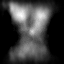
\includegraphics[width = 1in]{images/1-saliency.png}} \\
\subfloat{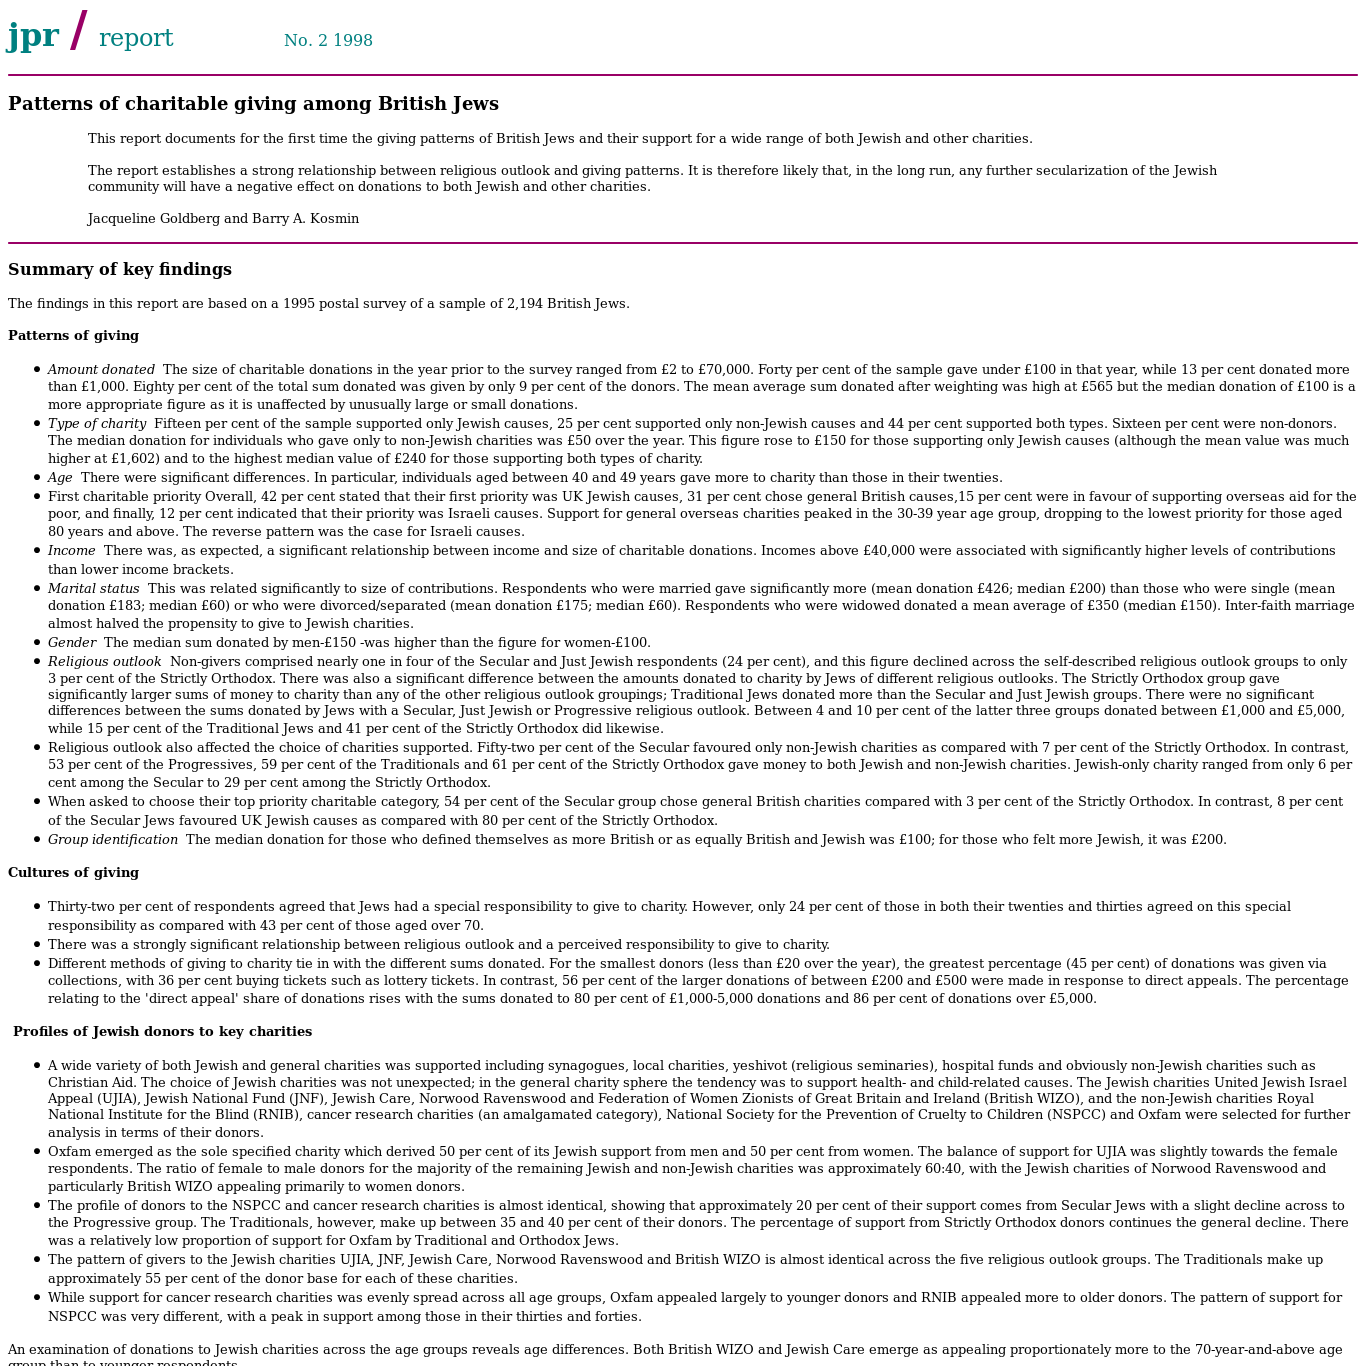
\includegraphics[width = 1in]{images/2-snapshot.png}} &
\subfloat{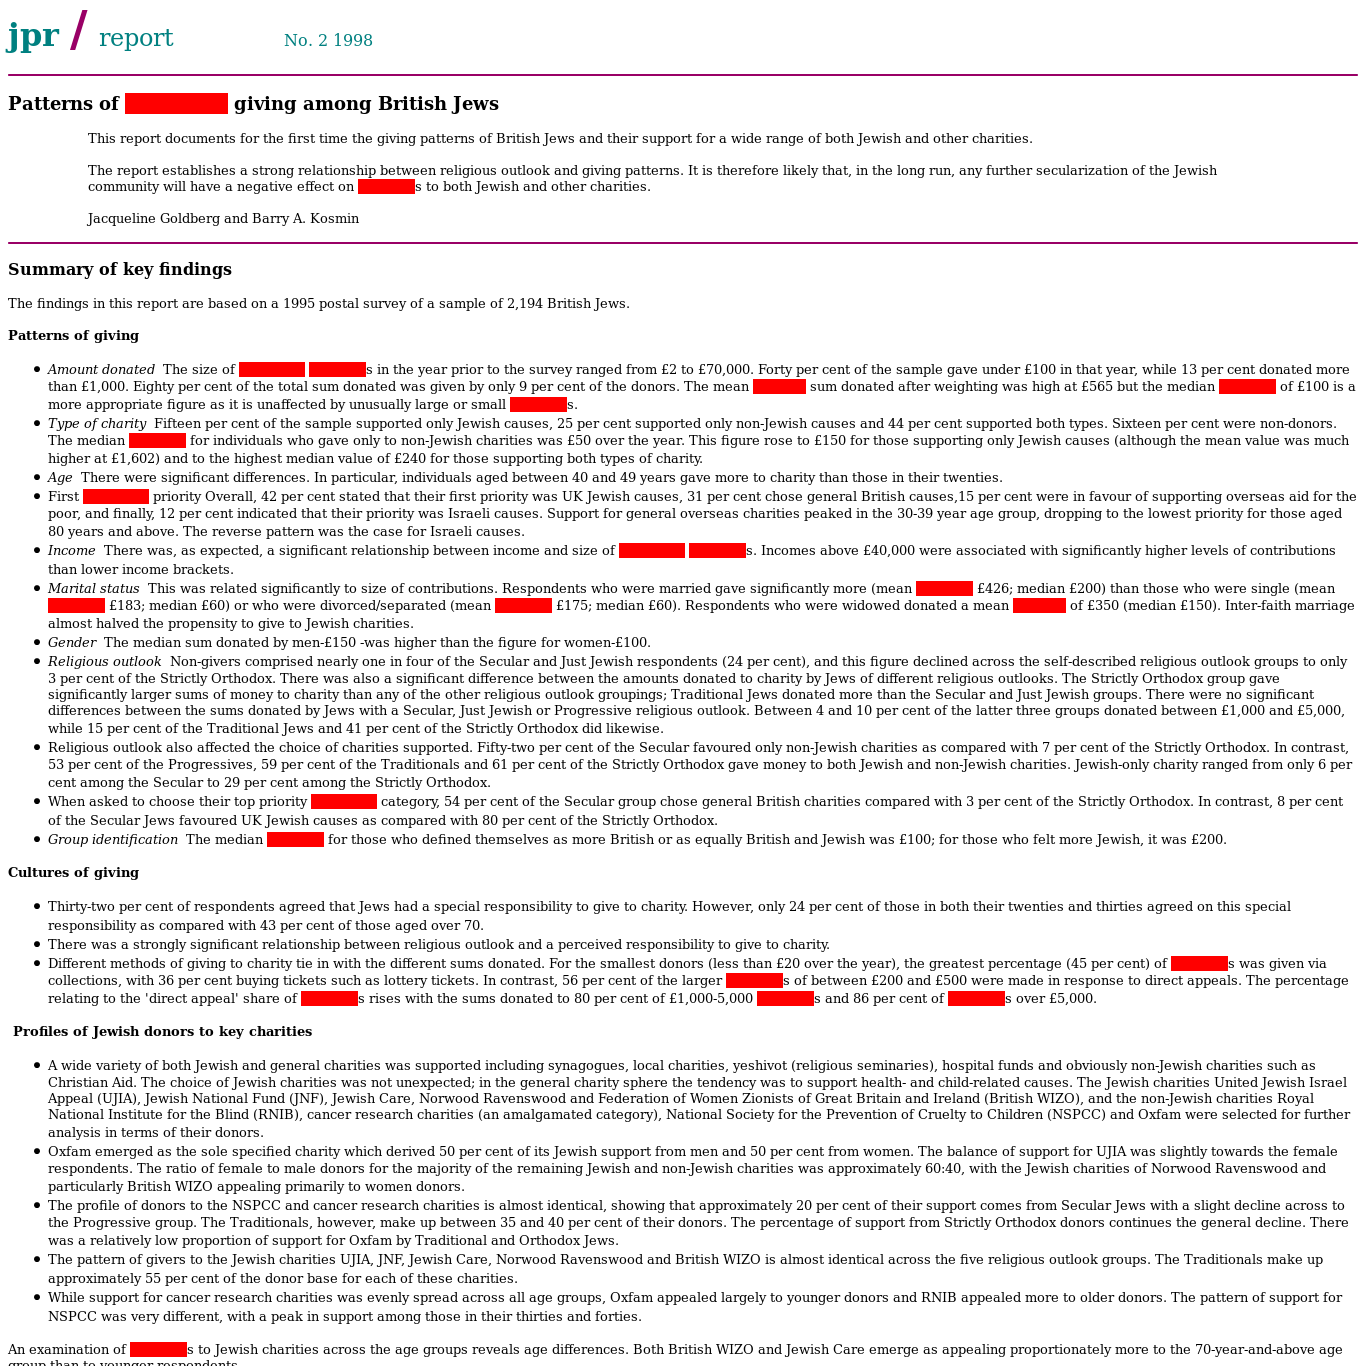
\includegraphics[width = 1in]{images/2-highlights.png}} &
\subfloat{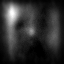
\includegraphics[width = 1in]{images/2-saliency.png}} \\
\subfloat{
\includegraphics[width = 1in]{images/3-snapshot.png}} &
\subfloat{
\includegraphics[width = 1in]{images/3-highlights.png}} &
\subfloat{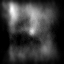
\includegraphics[width = 1in]{images/3-saliency.png}} \\
\end{tabular}
\caption{Examples of a vanilla snapshot, a red highlighted snapshot, and a saliency heatmap from left to right, respectively.}
\label{fig:exampleshots}
\end{figure}


%\subsubsection{Filtering}
\label{sec:datasetsum}
As the Wayback Machine does not contain an archived or working version of each document in the ClueWeb12 collection, a filtering process was introduced to maximize the quality of each snapshot. Using the following criteria, a snapshot was selected for each available document. 
\begin{enumerate}[nosep,leftmargin=14pt]
\item Each document is requested from the Wayback Machine. 
\item A document that is not on the Wayback Machine, times out, throws a JavaScript error or results in a PNG snapshot smaller than 100KB is marked as broken. Such documents are rendered again using the online rendering service provided by ClueWeb12.\footnote{\url{http://boston.lti.cs.cmu.edu/Services/}}
\item A manual selection is made between all documents that are rendered from both sources. The Wayback version is used if it contains more styling elements and if the content is the same as in the rendering service. Otherwise, the rendering service version is used. 
\end{enumerate}
%
As a result, most of the 28,906 judged documents had a corresponding snapshot from either the Wayback Machine or ClueWeb12 rendering service; only 265 documents did not pass the filtering and were discarded.
Table~\ref{tab:countsources}, row one, summarizes the results of the \datasetname~acquisition process.


\subsection{Non-visual features} 
\label{sec:contentfeature}
In LTR, documents are ranked based on various types of features, such as content features (BM25), quality indicators (PageRank) and behavioral features (CTR).
In order to use \datasetname~to measure the effect of visual features, we also add a set of content features and quality indicators.
In preliminary experiments, we compared the effect of reducing the 46 features in LETOR~\cite{qin2010letor} to just the 11 features described in Table~\ref{tab:setdescription}.
As these features are relatively easy to compute and the experiments showed a minimal drop in performance, we decided to limit ourselves to these features for \datasetname.
Also note that behavioral features, such as CTR, are not available for the TREC Web Tracks.

The content features are computed by doing a full pass over the complete ClueWeb12 collection using Apache Spark.\footnote{\url{https://spark.apache.org/}}
\if0
$^{ }$\footnote{This took approximately 20 hours on 116 Hadoop worker nodes with 3 executor cores and 21Gb memory each.}
\fi
During this process an HTML parser (jsoup\footnote{\url{https://jsoup.org/}} in our case) extracts the title and content from the raw HTML.
Because the HTML structure in very large documents cannot be parsed efficiently by jsoup, all documents with more than one million tokens are ignored.
Using the Apache Spark implementation of TF and IDF, a sparse vector is obtained for each term in each document. Finally, the sparse vectors are loaded into a Python Pandas dataframe, which is used to compute the TF, IDF, TF-IDF and BM25 scores for each document-query pair.

Additionally, PageRank scores from the ClueWeb12 Related Data section\footnote{\url{https://lemurproject.org/clueweb12/related-data.php}} are added to each document.

Finally, the following modifications based on the features from LETOR 3.0~\cite{qin2010letor} are made to stabilize training:
\begin{enumerate}[nosep,leftmargin=14pt]
% \item IDF is calculates as follows: 
% $$IDF(q, D) = \sum_{t_i \in q} IDF(t_i, D) = \sum_{t_i \in t} \log \frac{|D| + 1}{DF(t_i) + 1}$$
% Where  $q_i$ and $t_i$ represent a list of all terms in a query and a single query term respectively. $D$ represents a list of all terms in a document with $|D|$ as its total length. $DF(t_i)$ is the document frequency for the given query term.  
\item Free parameters $k_1$, $k_3$ and $b$ for BM25 were set to $2.5$, $0$ and $0.8$, respectively. 
\item Because the PageRank scores are usually an order of magnitude smaller than all other scores, we multiply each value by $10^5$.
\item After all features are computed, the log is taken over the final results.
\item The logged features are normalized per query.  
\end{enumerate}

\begin{table}[h]
\centering
\captionof{table}{Non-visual features provided with \datasetname.}  \label{tab:setdescription} 
\begin{tabular}{rlrlrl}
\toprule
Id & Description & Id & Description & Id & Description    \\ 
\midrule
1  & Pagerank  & 5  & Content TFIDF  & 9  & Title IDF   \\
2  & Content length & 6  & Content BM25   & 10 & Title TFIDF   \\
3  & Content TF  & 7  & Title length & 11 & Title BM25  \\
4  & Content IDF & 8  & Title TF  & & \\
\bottomrule
\end{tabular}
\end{table}



%\textit{(This has not been done yet)} The TF and IDF scores were also calculated Anchor text extracted by \citet{hiemstra2010mapreduce} 
% Make a seperate section for snapshots and subsections for collection, cleaning, statistics etc.


\subsection{Final collection}\label{sec:finalcollection}
In summary, \datasetname~contains:
\begin{inparaenum}[(i)]
\item a directory with web page snapshots (Section~\ref{sec:screenshotsec}), and
\item a set of files with content features divided into folds (Section~\ref{sec:contentfeature}).
\end{inparaenum}
%\todo{Why do we have a set of files with features and not only one file?}
Each snapshot is stored as a PNG file that can be identified by its corresponding ClueWeb12 document id. 
The non-visual features are stored in LETOR formatted files containing the raw, logged and query normalized values.
The query normalized values are randomly split per query into five equal partitions.
These partitions are then used to create five folds, where each fold contains three partitions for training and the remaining two partitions for validation and testing.

%A separate file contains an entry for each snapshot indicating whether the snapshots was created using the Wayback Machine or online rendering service. 

%\begin{figure*}[t]
%\centering
%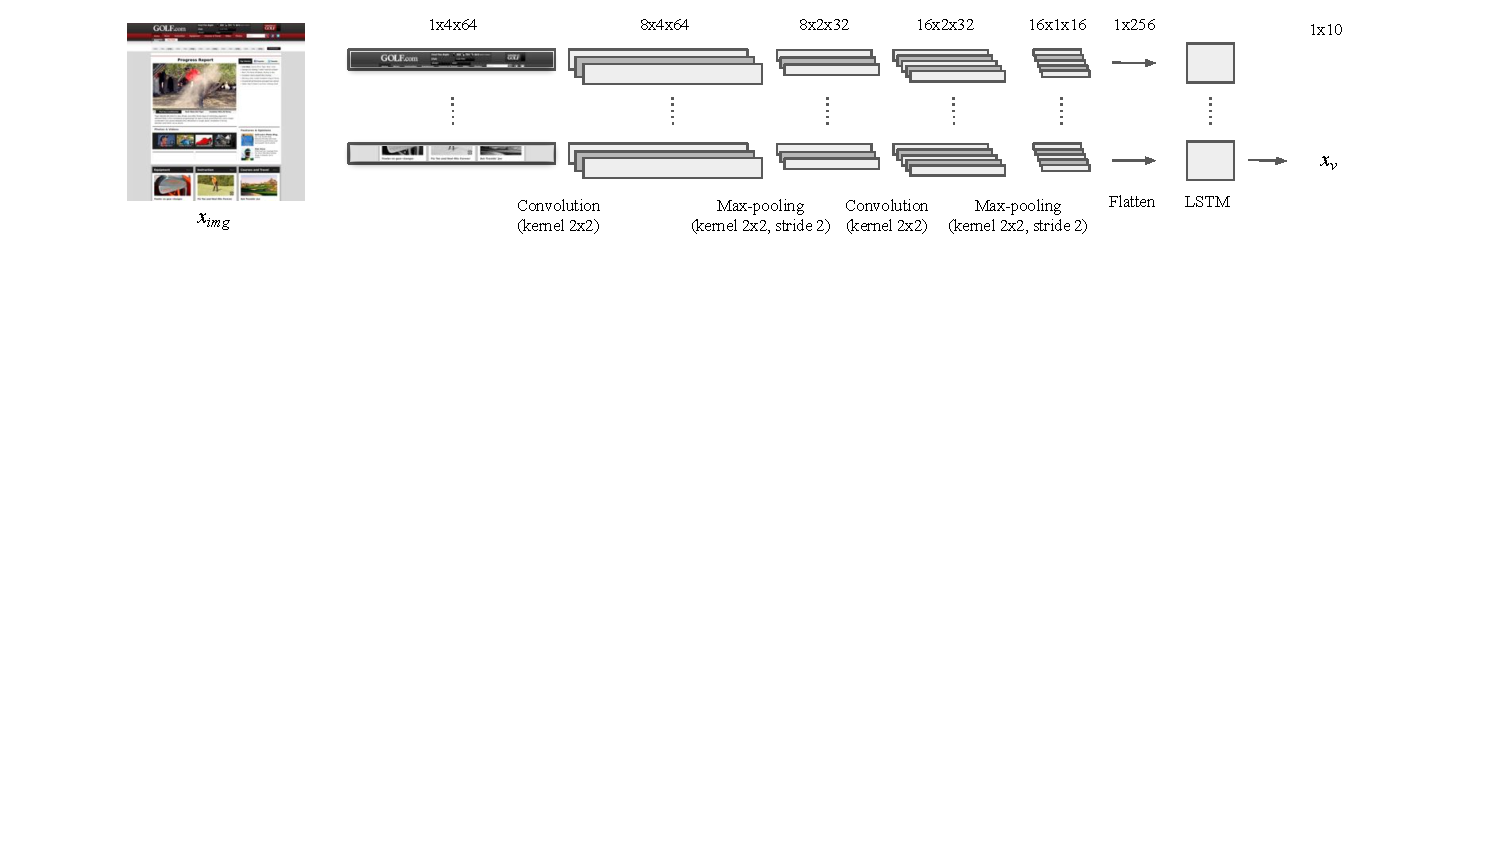
\includegraphics[clip,trim=0 10cm 0 0, width=20cm]{images/vip-features.pdf}
%  \captionof{figure}{The feature extractor architecture with corresponding dimensions used in our implementation of the ViP model.} \label{fig:ViPfeat} 
%\end{figure*}
